\documentclass[11pt]{report}
% PACKAGES
  \usepackage[a4paper,left=28mm,right=28mm,top=30mm,bottom=30mm]{geometry}
  \usepackage{graphicx,epstopdf}      % Used to import external graphics (figures)
  \usepackage{hyperref}       % Used for referring to links inside and outside the document
  \usepackage[table]{xcolor}  % To include colors 
  \usepackage{amsmath}        % For most of the math symbols and environments (such as \begin{align})
  \usepackage{amssymb}        % For using symbols in the document
  \usepackage{float}          % Arranging of figures on the page
  \usepackage[bf]{caption}    % Arranging the captions in floating environments [bf] makes the Figures bold
  \usepackage{subcaption}     % To arrange captions of subfigures
  \usepackage{booktabs}       % For standard tabular tables, with rules
  \usepackage{tabularx}       % For clean tables such as in the Nomenclature
  \usepackage{fancyhdr}       % Fancy headers
  \usepackage[colorinlistoftodos]{todonotes}      % To create todo notes
  \usepackage[nottoc,notlot,notlof]{tocbibind}    % Add bibliography to content
  \usepackage{bm}             % Make bold symbols
  \usepackage{lipsum}
  \usepackage{parskip}
  \usepackage[export]{adjustbox}
  \usepackage{changepage}
  \usepackage{pdfpages}
% LAY-OUT
  % \usepackage{pdfpages}

  % \usepackage{pdflscape}

   \renewcommand\thesection{\arabic{section}}

  % \usepackage[mathletters]{ucs}
  % \usepackage[utf8x]{inputenc}
  %Bibliography for references, with reference style options
  \usepackage[
  backend=biber,
  bibstyle=ieee,
  citestyle=numeric-comp,
  dashed=false,
  url = false,
  maxnames=8,
  maxcitenames=2,
  mincitenames=1,
  sorting=none,
  isbn = false,
  doi = false
  ]{biblatex}
  \addbibresource{references.bib}

  %Set the page style
  \pagestyle{fancy}
  \fancyhead[L]{\ifodd\value{page} \slshape\nouppercase{\rightmark} \else \fi}
  \fancyhead[R]{\ifodd\value{page} \else \slshape\nouppercase{\leftmark} \fi}
  \chead{ }
  \lfoot{}
  \rfoot{}
  \cfoot{\small\thepage}


  %Give colors to links/refs etc
  \hypersetup{colorlinks, linkcolor={blue!0!black}, 
                          citecolor={blue!70!black}, 
                           urlcolor={blue!80!}} 
                       
  %% Set up numbering and spacing
  \numberwithin{equation}{section}        %Number the equations per section
  \numberwithin{figure}{section}          %Number the figures per section
  \numberwithin{table}{section}           %Number the tables per section
  \captionsetup[table]{skip=1pt}          %Skip 1 pt after a table
  \captionsetup[figure]{skip=3.5pt}       %Skip 4 pt after a figure
  \setcounter{secnumdepth}{3}             %Count up to the subsubsection 
  \setcounter{topnumber}{1}               %Number of floats at top of a page (default is 2)

  %%%%% proof/theorem/definition boxes

  \usepackage{cleveref}
  \usepackage[most]{tcolorbox}
  \newtcbtheorem{Theorem}{Theorem}{
    enhanced,
    sharp corners,
    attach boxed title to top left={
      yshifttext=-1mm
    },
    colback=white,
    colframe=blue!75!black,
    fonttitle=\bfseries,
    boxed title style={
      sharp corners,
      size=small,
      colback=blue!75!black,
      colframe=blue!75!black,
    } 
  }{thm}

  \newtcbtheorem{Definition}{Definition}{
    enhanced,
    sharp corners,
    attach boxed title to top left={
      yshifttext=-1mm
    },
    colback=white,
    colframe=blue!25,
    fonttitle=\bfseries,
    coltitle=black,
    boxed title style={
      sharp corners,
      size=small,
      colback=blue!25,
      colframe=blue!25,
    } 
  }{def}

  \newtcbtheorem[no counter]{Proof}{Proof}{
    enhanced,
    sharp corners,
    attach boxed title to top left={
      yshifttext=-1mm
    },
    colback=white,
    colframe=blue!25,
    fonttitle=\bfseries,
    coltitle=black,
    boxed title style={
      sharp corners,
      size=small,
      colback=blue!25,
      colframe=blue!25,
    } 
  }{prf}
% DEFINITIONS
  %% Titlepage definitions
  \newcommand{\deltitle}{Impact-Aware Control for a Dual-Arm Setup}      %Your project title
  \newcommand{\StudentName}{Gijs van den Brandt}  %Student name
  \newcommand{\StudentID}{1257110}                    %Your student number
  % \newcommand{\DCcode}{2021.109}                      %Get your DC code from the D&C secretariat

  %% Operators
  \DeclareMathOperator\sign{sgn}                      %Sign function
  \DeclareMathOperator\diag{diag}                     %Diagonal operator
  \DeclareMathOperator\imag{Imag}                     %Imaginary part of complex variable
  \DeclareMathOperator\real{Real}                     %Real part of complex variable
  \DeclareMathOperator*{\argmin}{\arg\!\min}          %Argmin operator
  \newcommand{\norm}[1]{\left\lVert#1\right\rVert}    %Norm operator

  %% Variable definition
  \newcommand{\R}{\mathbb{R}}                         % Set of real numbers
  \newcommand{\C}{\mathbb{C}}                         % Set of complex numbers

\begin{document}

% Summary 
  \section*{Progress meeting 13 | 6 December, 2022}


  \section*{1. Progress}
  \begin{itemize}
  \item \textbf{Controller finishing touches:}
      \begin{itemize}
        \item The controller now uses feedforward, which improves tracking prior to the impact. To achieve this, the impedance force during the demonstration is recorded and applied as feedforward during the replay.
        \item The impedance stiffness during replay was increased from 800 N/m to 1500 N/m. The stiffness during demonstration remains at 800 N/m. Combined with the feedforward, this causes the position tracking during the stamping task to decrease from approx. 20 mm to 3 mm prior to impact.
        \item Previously, reference spreading was only applied for the translational DoFs. I have now extended this so that reference spreading also works for the rotational DoFs.

      \end{itemize}
      
      \item \textbf{Data collection:} The stamping and grabbing experiment I showed in the previous progress report were repeated with the modified controller. Based on your feedback, this time I did stamping experiments where the impact surface was lowered, raised, or kept equal. Furthermore I recorded videos of the experiments.

      During the previous progress meeting, the results caused a bit of confusion; the surface was raised, yet the impact occured later due to poor tracking. Feedforward and higher gains solved this issue. The conclusions that can be drawn from the experiments did not change with respect to last time. The videos and figures are available at \url{https://surfdrive.surf.nl/files/index.php/s/3FMyF4ZadnimjsO}. In section \ref{sec:2}, two selected figures are shown: one for the stamping experiment where the surface was raised, and for box grabbing.

      \item \textbf{Writing:} Jari advised me to focus on determining the structure of my paper, rather than jumping straight into writing the individual sections. Section \ref{sec:1} shows what I have in mind. The paper in its current state is attached at the end of this document. 

     
  \end{itemize}

  \section*{2. Agenda}
  During the meeting, I would like to discuss the following points:
  
      \begin{itemize}
        \item In my opinion, the new experimental results demonstrate the value of reference spreading. Nevertheless, I think that reference spreading would be more effective with faster impact detection, which I think could be achieved by a momentum observer with different tuning from the tuning provided by franka emika. Do you think that I should spend time on a momentum observer, or spend more time on other changes to the controller? Or do you think that the results are already sufficiently convincing?
  \item I would like to go over the paper structure I have in mind. Jari has already given me some advice regarding what a paper should look like, however we came to the agreement that my final report should be somewhere between a paper and a thesis (to give an example, the custom end effector design wouldn't be considered a scientific contribution in an academic paper, whereas in a thesis report I believe it shouldn't be hidden in an appendix). I am curious to hear your opninion on this.
  \item I have made a planning for when I want to the send the report to you for feedback, and when I hope to receive the feedback. I want to ask if this planning seems reasonable to you.
  \end{itemize}

  \section*{3. Next steps}

  \begin{itemize}
      \item Make figures: error peaking, reference spreading, VR control loop with human, photo of setup, ...
      \item Document math: reference extending (also for rotations), impact detection, ...
      \item Finish draft of paper for feedback. Some major components that should still be written: teleoperation, custom end effector, experimental results, conclusion.
      \item (Low priority for now: document controller code so that it may be used by others in the future)
  \end{itemize}

  \section*{4. Long-term planning}
  Shown below is the current long-term planning for the project phase. It includes deadline, such as when I intend to submit the report for feedback. I received a deadline extension, meaning that the final deadline is the 5th of March. I plan for a defence around the 20th of February.

  \begin{figure}[H]
  \centering
  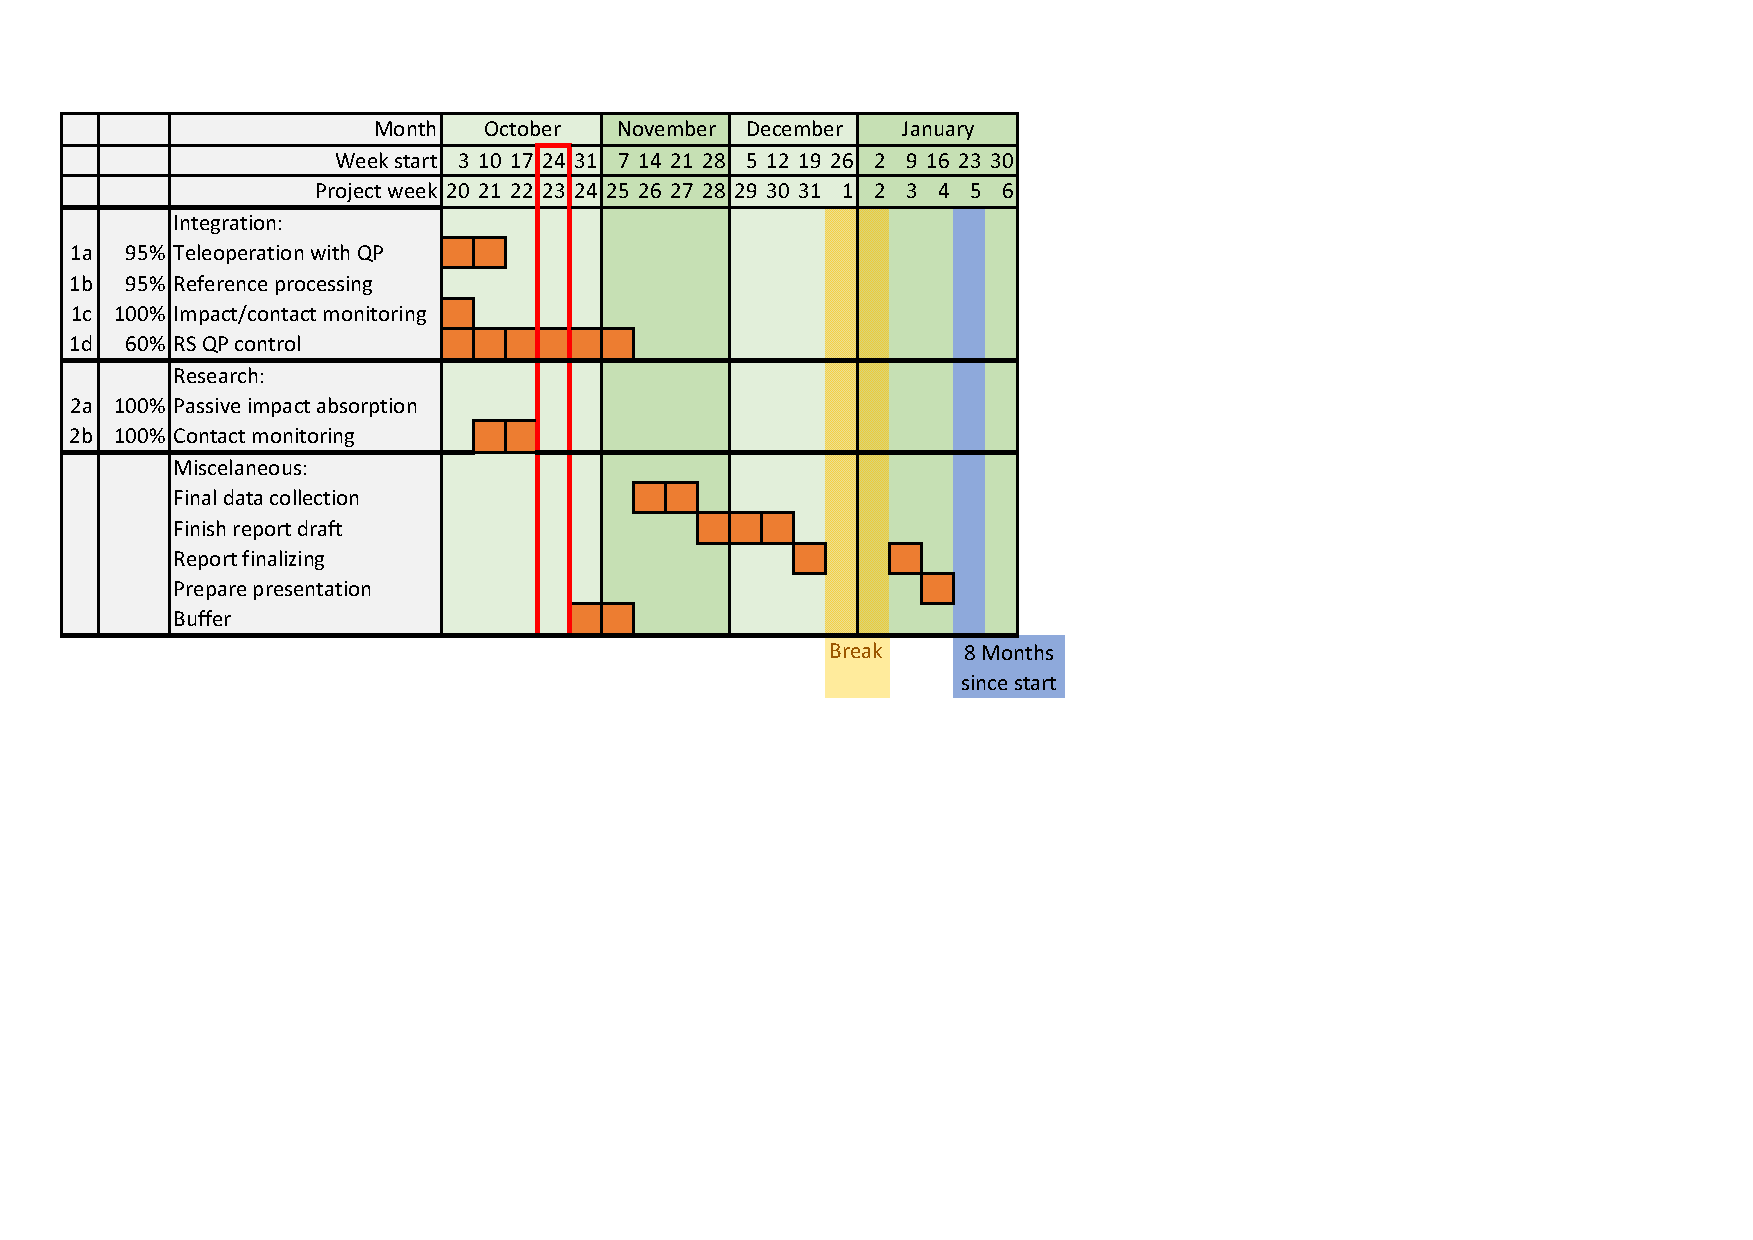
\includegraphics[width=\textwidth, trim={0.87cm 6.5cm 4.5cm 1.5cm},clip]{Graphics/planning v2.pdf}

  \label{fig:my_label}
  \end{figure}

  \begin{enumerate}
  \item[1a] \textbf{Translating dual-arm teleoperation to the physical setup.} The existing implementation in simulation already uses the mc\_rtc interface, meaning that the switch to reality shouldn't pose an issue. Nevertheless, this step also involves getting familiar with the software, which increases the anticipated time for this step.
  \item[1b] \textbf{Extracting references from the demonstration data.} The demonstrated trajectories should be split into ante-impact and post-impact sections, and extended to facilitate RS. Furthermore multiple measurements should be used to fit ProMPs, after which a reference can be generated. It is also key to identify which data should be learned from the demonstration. This is not limited to choosing between a force or position reference, but can also consists of learning properties of the environment, e.g. friction cones or box inertia, that are crucial to a dual-arm box grabbing scenario.
  \item[1c] \textbf{Integrating impact detection and contact monitoring in mc\_rtc.} The majority of the impact detector's complexity resides in the momentum observer; however, Franka Emika's software already has an integrated momentum observer. This still leaves tuning of the impact detecting algorithms which might be time consuming. Furthermore an analysis comparing the available methods could be worthwhile. Factors which determines the effectivity of the impact detection algorithm include speed of detection, as well as reliability, i.e. the rate of false positives. The addition of objects that cause unexpected impacts is not considered a part of the research scope.
  \item[1d] \textbf{Configuring QP controllers for the ante-impact, intermediate, and post-impact phase.} For each of the phases, it is important to address the redundancy in the arms' degrees of freedom. After that, control for the ante-impact phase should be trivial. For the intermediate phase, it is expected that ante-impact reference tracking without velocity feedback should be applicable on a dual-arm robot, though this might prove to be false, in which case other methods should be investigated. During post-impact control, the challenge will be maintaining non-slip contact with the box. It is difficult to say how well the results from simulations can be repeated with torque control, where the state of the box can not be sensed to be used in the QP controller.
   \item[2a] \textbf{Passive impact absorption:} A soft cover for the end effector will be designed. Such a cover can be connected to the Panda by connecting bolts to the so-called flange interface. A mold will be created using 3D printing to allow for casting of various silicone soft covers. Design parameters -- i.e. material properties (controlled by choosing different kinds of silicone) and soft cover thickness -- will be analyzed experimentally. A systematic comparison between various designs will require an experiment plan including a realistic testing scenario. Evaluation of performance can be based on the oscillatory response in position and force after establishing contact. Furthermore multiple scenarios with various box surface properties and robot poses should be considered.
  
  \item[2b] \textbf{Contact monitoring:} When investigating contact monitoring, two approaches can be taken: either using proprioceptive or exteroceptive sensors. A possible improvement for contact monitoring using proprioceptive sensors could be to wait a fixed time starting from the last detected impact, rather than waiting a fixed time from the first impact. As for exteroceptive sensors, they can be a hurdle for large-scale commercial applications as they are not integrated in the robot. However, if a soft cover is to be mounted to the end effector, including tactile sensors for impact and contact monitoring becomes more feasible. Practical questions such as which tactile sensor to use and how to integrate it could be addressed, though this is not absolutely necessary for completing the research goals, and therefore has a low priority.
  \end{enumerate}
% main text
\newpage
  \section{Paper structure}\label{sec:1}
  Below is the structure of the paper that I have in mind. The current stat of the paper is attached at the end of this document.

   Title: Experimental Validation of Reference Spreading for Robotic Manipulation of Unmodeled Objects
\begin{enumerate}
      \item Introduction

      \item System overview
\begin{enumerate}
      \item  Robot dynamics
      \item Task description (box weight/dimension, explanation of stamping and grabbing)
 \end{enumerate}
      \item Soft end effector design

      \item Trajectory planning using teleoperation
\begin{enumerate}
     \item  VR device

       \item  Impedance controller
\end{enumerate}
      \item Reference spreading
\begin{enumerate}
       \item  Impact detection

      \item  Reference formulation

       \item  Switching controller
\end{enumerate}
     \item  Experimental results
\begin{enumerate}
       \item  Stamping task

      \item  Grabbing task

       \item  (don’t think I should do more complicated tasks as they require more explanation while not showing additional benefits of RS)
      \end{enumerate}
     \item   Conclusion
    
     \item  Future work


\end{enumerate}
Appendix:

A.  End effector design: complete technical drawing and manufacturing process

B.  Experimental results: Can’t show all the data in the main text (probably only one or two direction, e.g. downward direction for stamping). Include full results in appendix.

C.  Math regarding rotation matrices and quaternions: definition of rotation error, interpolation of quaternions, integrating angular velocity for extending the rotation reference.

  \newpage

  \section{Selected figures of experimental results}\label{sec:2}
  (see following pages)
\begin{figure}[]
  \centering
  \begin{adjustwidth}{0pt}{5pt}
  \centering
  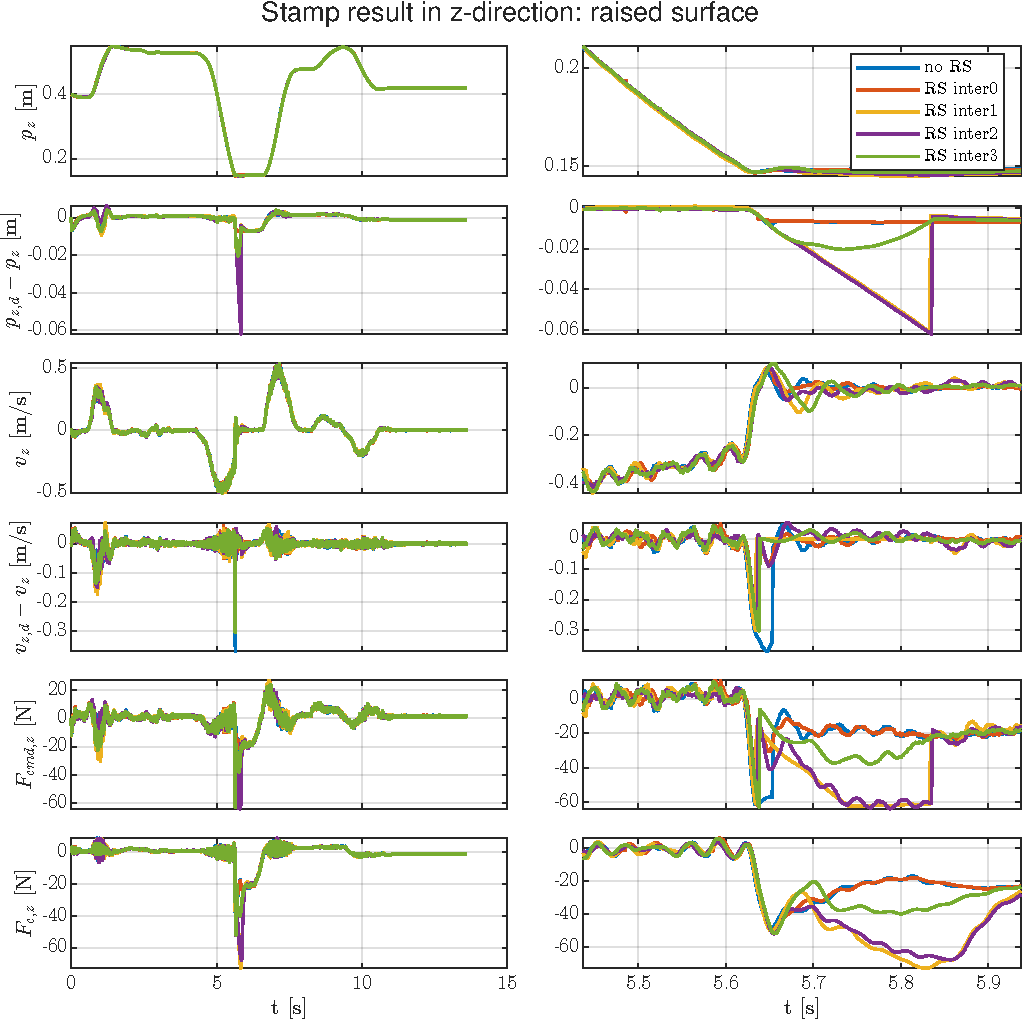
\includegraphics[width=0.75\textwidth]{Graphics/Stamp result in z-direction raised surface.pdf}\\
    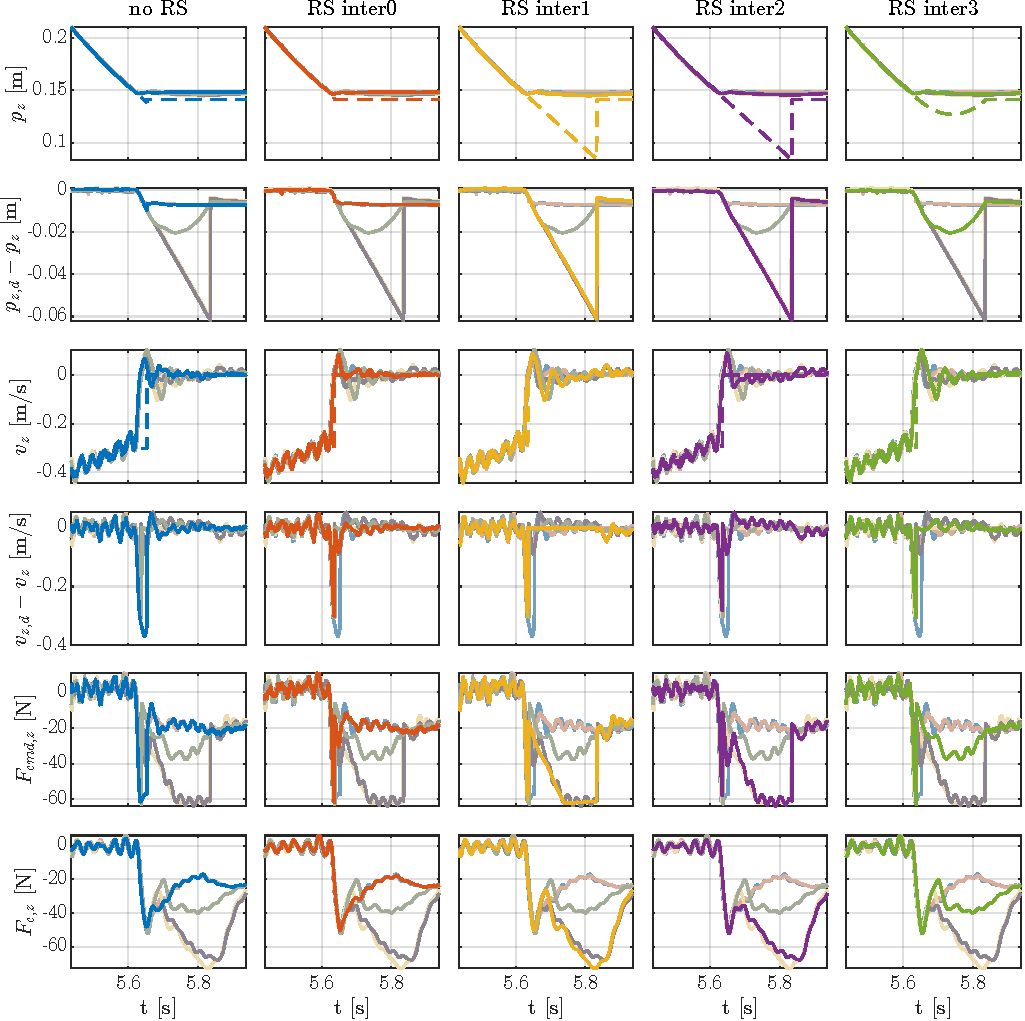
\includegraphics[width=0.75\textwidth]{Graphics/Stamp result in z-direction raised surface_.pdf}
  \end{adjustwidth}
  \caption{Results of a stamping experiment. The top figure shows the results for the various approaches, both over the entire experiment, and over a small timeframe around the impact. The bottom figure isolates each approach for additional clarity. The dotted lines indicate the target as described in the control approaches.}
  \label{fig:stamp}
  \end{figure}

\begin{figure}[]
  \centering
  \begin{adjustwidth}{0pt}{5pt}
  \centering
  \includegraphics[width=0.75\textwidth]{Graphics/Grab result in y-direction_ Panda1.pdf}\\
    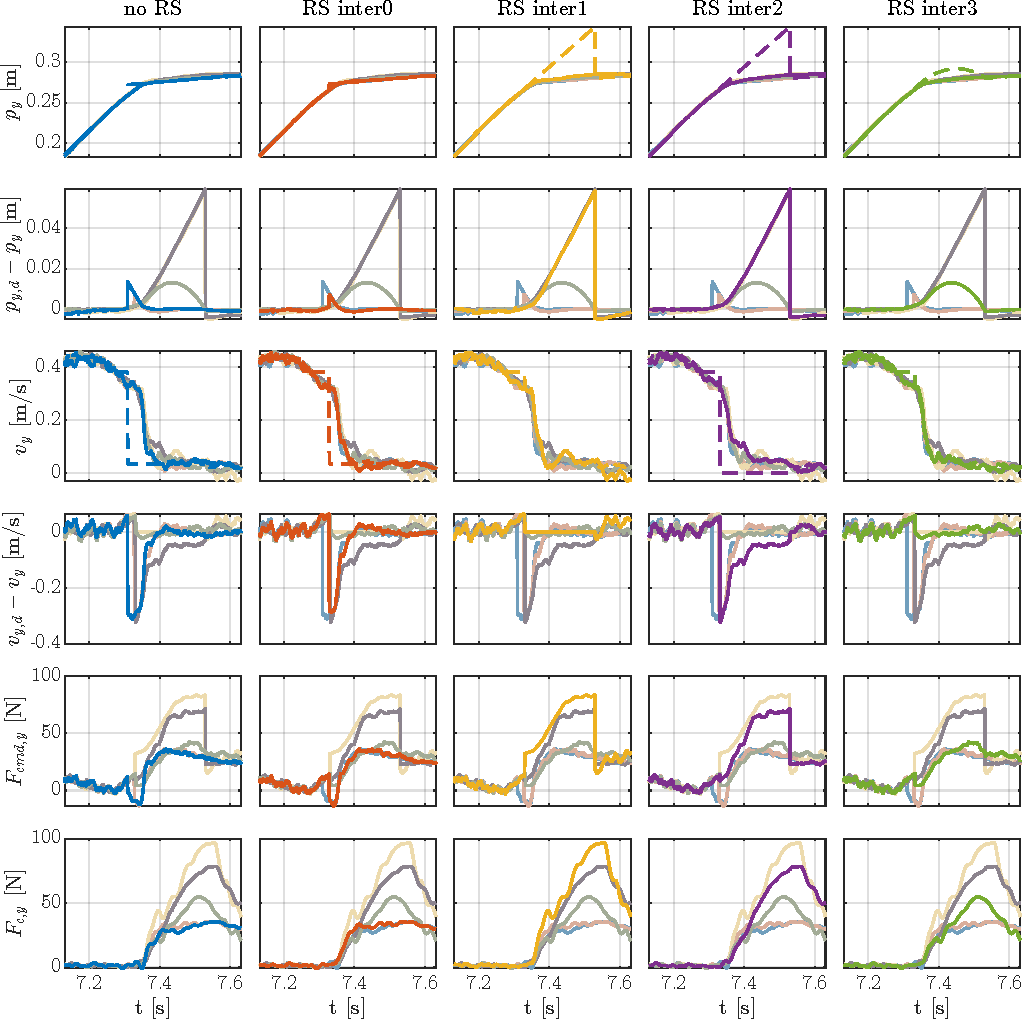
\includegraphics[width=0.75\textwidth]{Graphics/Grab result in y-direction_ Panda1_.pdf}
  \end{adjustwidth}
  \caption{Results of arm 1 in boxgrab experiment.}
  \label{fig:grab1}
  \end{figure}



  \newpage
  % 
% Setup
    \documentclass[a4paper, 10pt, conference]{ieeeconf}
    \IEEEoverridecommandlockouts                              % This command is only
                                                              % needed if you want to
                                                              % use the \thanks command
    \overrideIEEEmargins
    % See the \addtolength command later in the file to balance the column lengths
    % on the last page of the document

    \usepackage[utf8]{inputenc}
    \usepackage[T1]{fontenc}

    \usepackage[
bibstyle=ieee,
isbn = false,
doi = false,
url = false,
eprint=false]{biblatex}


\AtEveryBibitem{\clearfield{address}}
\AtEveryBibitem{\clearlist{language}}

\addbibresource{refs.bib}

\DefineBibliographyStrings{english}{
  phdthesis   = Ph\adddot D\adddot\addspace thesis,
  mathesis    = Master's thesis,
}

% https://ftp.snt.utwente.nl/pub/software/tex/macros/latex/contrib/biblatex-contrib/biblatex-ieee/ieee.bbx

%swapped chapter+pages with published+location date:

\DeclareBibliographyDriver{inproceedings}{%
  \usebibmacro{bibindex}%
  \usebibmacro{begentry}%
  \usebibmacro{author/translator+others}%
  \setunit{\labelnamepunct}\newblock
  \usebibmacro{title}%
  \newunit
  \printlist{language}%
  \newunit\newblock
  \usebibmacro{byauthor}%
  \newunit\newblock
  \usebibmacro{maintitle+booktitle(inproceedings)}%
  \midsentence
  \newunit\newblock
  \usebibmacro{event+venue+date}%
  \newunit\newblock
  \usebibmacro{byeditor+others}%
  \newunit\newblock
  \printfield{volumes}%
  \newunit\newblock
  \usebibmacro{series+number}%
  \newunit\newblock
  \printfield{note}%
  \newunit\newblock
  \printlist{organization}%
  \newunit\newblock
  \usebibmacro{volume+part}%
  \newunit\newblock
  \usebibmacro{chapter+pages}% %swapped chapter+pages with published+location date
  \newunit
  \usebibmacro{publisher+location+date}%
  \newunit\newblock
  \iftoggle{bbx:isbn}
    {\printfield{isbn}}
    {}%
  \newunit\newblock
  \usebibmacro{doi+eprint+url}%
  \newunit\newblock
  \usebibmacro{addendum+pubstate}%
  \setunit{\bibpagerefpunct}\newblock
  \usebibmacro{pageref}%
  \newunit\newblock
  \iftoggle{bbx:related}
    {\usebibmacro{related:init}%
     \usebibmacro{related}}
    {}%
  \usebibmacro{finentry}}
  
  
  %swapped chapter+pages with published+location date:
  
  \DeclareBibliographyDriver{incollection}{%
  \usebibmacro{bibindex}%
  \usebibmacro{begentry}%
  \usebibmacro{author/translator+others}%
  \setunit{\labelnamepunct}\newblock
  \usebibmacro{title}%
  \newunit
  \printlist{language}%
  \newunit\newblock
  \usebibmacro{byauthor}%
  \newunit\newblock
  \usebibmacro{in:}%
  \usebibmacro{maintitle+booktitle}%
  \newunit\newblock
  \usebibmacro{series+number}%
  \newunit\newblock
  \usebibmacro{byeditor+others}%
  \newunit\newblock
  \printfield{edition}%
  \newunit
  \iffieldundef{maintitle}
    {\printfield{volume}%
     \printfield{part}}
    {}%
  \newunit
  \printfield{volumes}%
  \newunit\newblock
  \printfield{note}%
  \newunit\newblock
  \usebibmacro{chapter+pages}%
  \newunit\newblock
  \usebibmacro{publisher+location+date}%
  \newunit\newblock
  \iftoggle{bbx:isbn}
    {\printfield{isbn}}
    {}%
  \newunit\newblock
  \usebibmacro{doi+eprint+url}%
  \newunit\newblock
  \usebibmacro{addendum+pubstate}%
  \setunit{\bibpagerefpunct}\newblock
  \usebibmacro{pageref}%
  \newunit\newblock
  \iftoggle{bbx:related}
    {\usebibmacro{related:init}%
     \usebibmacro{related}}
    {}%
  \usebibmacro{finentry}}


    % The following packages can be found on http:\\www.ctan.org
    \usepackage{graphics} % for pdf, bitmapped graphics files
    \usepackage{epsfig} % for postscript graphics files
    \usepackage{mathptmx} % assumes new font selection scheme installed
    \usepackage{mathptmx} % assumes new font selection scheme installed
    \usepackage{amsmath} % assumes amsmath package installed
    \usepackage{amssymb}  % assumes amsmath package installed

    \title{\LARGE \bf
    Experimental Validation of Reference Spreading for Robotic Manipulation of Unmodeled Objects
    }

    %\author{ \parbox{3 in}{\centering Huibert Kwakernaak*
    %         \thanks{*Use the $\backslash$thanks command to put information here}\\
    %         Faculty of Electrical Engineering, Mathematics and Computer Science\\
    %         University of Twente\\
    %         7500 AE Enschede, The Netherlands\\
    %         {\tt\small h.kwakernaak@autsubmit.com}}
    %         \hspace*{ 0.5 in}
    %         \parbox{3 in}{ \centering Pradeep Misra**
    %         \thanks{**The footnote marks may be inserted manually}\\
    %        Department of Electrical Engineering \\
    %         Wright State University\\
    %         Dayton, OH 45435, USA\\
    %         {\tt\small pmisra@cs.wright.edu}}
    %}

    \author{Gijs van den Brandt% <-this % stops a space
    % \thanks{*This work was not supported by any organization}% <-this % stops a space
    % \thanks{$^{1}$H. Kwakernaak is with Faculty of Electrical Engineering, Mathematics and Computer Science,
    %         University of Twente, 7500 AE Enschede, The Netherlands
    %         {\tt\small h.kwakernaak at papercept.net}}%
    % \thanks{$^{2}$P. Misra is with the Department of Electrical Engineering, Wright State University,
    %         Dayton, OH 45435, USA
    %         {\tt\small p.misra at ieee.org}}%
    }


    \begin{document}



    \maketitle
    \thispagestyle{empty}
    \pagestyle{empty}

% Abstract
    \begin{abstract}

    This electronic document is a ``live'' template. The various components of your paper [title, text, heads, etc.] are already defined on the style sheet, as illustrated by the portions given in this document.

    \end{abstract}

% Introduction
    \section{INTRODUCTION}

    Automation has historically played a crucial role in the logistics industry. Our current way of living depends on autonomous systems for global transportation and warehousing. The growing labor shortage and increasing demand for online retail motivate further developments in the logistics sector~\cite{dekhneAutomationLogisticsBig2019}.

    A logistical aspect where machines struggle to fully compete with humans is object manipulation. Practical examples of this include order picking or depalletizing. While robots are strong and consistent when manipulating objects, humans are versatile and swift. Robots are held back from faster performance because they must often slow down prior to making contact; establishing contact at a high velocity -- an event referred to as an impact -- could cause damage to the robot or its environment. On the contrary, humans intrinsically exploit impacts in the form of grabbing, bouncing and hitting.

    The field of impact-aware control aims to better equip robots for making contact at high velocities. These impacts are paired with large contact forces that could damage the system. Previous work describes control using the maximum allowable impact velocity that complies with safety constraints such as limits for the contact force~\cite{dehioRobotSafeImpactsSoft2021, dehioDualArmBoxGrabbing2022}. This was combined with a compliant cover for the robot that reduces contact forces at impact, facilitating higher feasible impact velocities. Rather than using a soft cover, compliancy may also be achieved by designing a robot with low inertia and high backdrivability as was done in \cite{songDevelopmentLowInertiaHighStiffness2018}.

    In addition to the large contact forces, a subject of interest is the velocity jump at the time of impact. Time misalignments between velocity jumps in the reference and in the actual system cause the velocity tracking error to peak\cite{biemondTrackingControlMechanical2012}, as is shown in Figure xxx. This error peak results in undesired control effort and should therefore be avoided. In \cite{yangImpactInvariantControl2021}, the robot's velocities are projected into an impact-invariant subspace based on the expected point of impact. As a result, impact-driven peaks in the velocity tracking error are reduced significantly. It is not always possible to describe a point of impact, however. Often times, impacts occur between surfaces rather than just points. Furthermore, corners of the surface may impact at diverging intervals in uncertain order during what is called near-simultaneous impacts, shown in Figure xxx.

    The impact-aware control scheme called Reference Spreading \cite{sacconSensitivityAnalysisHybrid2014} addresses error peaking caused by misaligned impacts. It operates on the basis of a tracking error that switches once an impact is detected. This concept is best explained at the hand of Figure xxx. The reference is split at the nominal impact time into an ante- and post impact reference. These references are then extended. Initially, the tracking error is based on the extended ante-impact reference, but this is switched to the post-impact reference once an impact is detected. Evidently, this can reduce the error peaking.

    Reference spreading can also handle simultaneous impacts. \cite{vansteenRobotControlSimultaneous2021} (explanation)

    By addressing the peaking error, reference spreading facilitates faster object manipulation, making it interesting to industry if its effectivity can be proven in practice. Reference spreading for object manipulation has already been validated in simulations \cite{vansteenRobotControlSimultaneous2021,zwartImpactAwareLearningDemonstration2019}. Experimental validations have been limited to interaction with a fixed environment, however \cite{rijnenReferenceSpreadingTracking2020,uitendaalTeachingRobotsInteraction2022}. The goal of this work is therefore to \textbf{provide a real-world implementation of reference spreading for practical object manipulation tasks.} To translate the results from simulation to reality, the following contributions are made:

    \textbf{1. Motion planning for impacts without object models}: Generating a reference with velocity jumps that is coherent with the system’s dynamics is challenging. 
    One approach maps the ante-impact velocity to the post-impact velocity based on conservation of momentum [ref for impact map]. This requires a model of the environment, which is feasible in simulations with simplified dynamics, but challenging in reality.
    Impact-driven velocity jumps could instead be inferred experimentally. In previous studies \cite{aouajPredictingPostImpactVelocity2021}, the control gains are reduced to zero upon detection of the impact while inferring an impact map, so that the velocity jump would not result in excessive motor torques.
    A different model-free motion planning strategy is proposed, which not only produces velocity-reference jumps that are coherent with the system dynamics, but also leverages human intuition to generate fluid motions before and after the impact. This is achieved by introducing a human in the loop by means of teleoperation. %(This strategy introduces a human in the loop by means of teleoperation; the operator performs a demonstration, after which a reference can be extracted. During the demonstration, the control gains are relatively low. This mitigates the torque jumps at the time of impact, meaning that the controller does not need to be turned off. The teleoperator instinctively accounts for the low control gains and can perform precise motion tasks despite poor tracking of the controller.)

    \textbf{2. Impact detection}: The reference spreading scheme should switch between ante-, intermediate-, and post-impact references at the appropriate time. This requires an impact detection algorithm. Approaches in literature look either at position data \cite{rijnenMotionSignalsVelocity2018} or external force estimations \cite{uitendaalTeachingRobotsInteraction2022,properAimAwareCollisionMonitoring2021,properValidationNumericalSimultaneous2022} for signs that could be caused by impacts. We show that these signs are necessary, but not sufficient conditions for an impact -- only looking at position or contact force can result in false positives. To limit false detection of impacts, a novel impact detector that looks at both force and position data is proposed and evaluated.

    \textbf{3. Custom end effector:}

    \textbf{4. Intermediate impact phase controller:}

% System overview
    \section{System overview}
    Considering the goal of evaluating reference spreading in a practical usecase, this work will focus on a dual-arm robotic setup. Having two arms increases the maximum payload. Furthermore, some object manipulation tasks, such as grabbing, require contact from multiple sides. The impact tasks that are considered in this work are stamping, swiping, grabbing, and tilting. 

    The Franka Emika robot \cite{haddadinFrankaEmikaRobot2022} is used for the setup as it is affordable and, more importantly, capable of torque control which is critical for impact-aware manipulation. The robot uses harmonic drives that inherently have poor backdriveability, however, torque control is still possible thanks to the torque sensors. 

    The system is limited in certain aspects to make it more representative of affordable setups in industry; in contrast to other object-manipulation works, we do not employ object pose estimation, environment models, or exteroceptive force/torque sensors. 

    \subsection{Robot dynamics}
    The robot dynamics can be described as 
    \begin{equation}
    M(q)\ddot{q}+h(q,\dot{q})= \tau_{cmd} + \sum_{i=1}^n J_i^Tf_{c,i}
    \end{equation}
    
    with inertia matrix $M$, joint accelerations $\ddot{q}$, centrifugal, coriolis and gravity terms $h$, and commanded torque $\tau_{cmd}$. The robot has $n$ contacts, and for each contact i there is an external contact wrench $f_{c,i}$. The wrench's contribution on joint level is related through contact jacobian $J_i$ for which it holds that $\begin{bmatrix} \omega & \dot{p} \end{bmatrix}_i^T=J_i\dot{q}$, with $\omega$ the angular velocities of the contact body and $\dot{p}$ the Cartesian velocities of the contact point. 

    For modeling purposes, it is assumed that contact forces only act on the end effector body. These forces are modeled as a single contact wrench $f_c$ acting on control point $p$, which is chosen as the intersection of robot link 5 and 7. This assumption allows for $f_c$ to be estimated using methods described in section xxx. Furthermore, omitting dependency on $q$ and $\dot{q}$ from for brevity results in

    \begin{equation}
    M\ddot{q}+h=\tau_{cmd}+J^Tf_c.
    \end{equation}

    \subsection{Base controller}
    For articulated robot arms, it is convenient to control the pose of the end effector in Cartesian space, rather than controlling the joint angles. This can be accomplished with an impedance controller.

    The desired impedance behavior is
    \begin{equation} \label{eq:impedance_desired}
     \Lambda  \begin{bmatrix} d_{\dot{\omega}} - \dot{\omega}   \\ d_{\ddot{p}} - \ddot{p}  \end{bmatrix} + D \begin{bmatrix}d_\omega - {\omega} \\ d_{\dot{p}} - \dot{p} \end{bmatrix}  + K \begin{bmatrix} e_{rot} \\d_p - {p}  \end{bmatrix} = d_{f_c} -f_c:
     \end{equation} 

    a mass spring damper with with Cartesian-space inertia, damping and stiffness matrices $\Lambda$, $D$ and $K$, and rotation tracking error $e_{rot}$ as defined in Appendix xxx. Desired values are denotes as $d_{(\cdot)}$, e.g., the desired value for $\ddot{p}$ is  $d_{\ddot{p}}$.

    Stiffness $K$ is typically chosen as a diagonal matrix. The damping matrix is determined following $D = 2(\Lambda K)^{\frac{1}{2}}$ which guarantees stable behavior when $K$ and $\Lambda$ are symmetric. Furthermore, For the inertia matrix, two options were considered. Choosing a diagonal matrix $\Lambda$ decouples the accelerations w.r.t. to the position error, resulting in better tracking in free motion. This approach was used in~\cite{vanoorschotDesignNumericalValidation2022}. In this work, however, the task-space inertia is set to match the joint-space inertia following $\Lambda^{-1} = JM^{-1}J^T$, decoupling the contact force w.r.t. the position error for better performance during contact. Further motivation for this decision is provided in Appendix xxx. % = \begin{bmatrix} e_{rotation} & e_{translation} \end{bmatrix}^T $. 

    Based on \ref{eq:impedance_desired} we can determine target task-space accelerations, $t_{\dot{\omega}}$ and $t_{\ddot{p}}$, following
    
    \begin{align} \begin{bmatrix}t_{\dot{\omega}}\\ t_{\ddot{p}}\end{bmatrix} &= \begin{bmatrix} {\dot{\omega}}\\{\ddot{p}}\end{bmatrix}+\Lambda^{-1} f_c\\
     &=     \begin{bmatrix} d_{\dot{\omega}}    \\ d_{\ddot{p}}  \end{bmatrix} +\Lambda^{-1} \left ( D \begin{bmatrix}d_\omega - {\omega} \\ d_{\dot{p}} - \dot{p} \end{bmatrix}  + K \begin{bmatrix} e_{rot} \\d_p - {p}  \end{bmatrix}- d_{f_c} \right ).
    \end{align}

    Note the exclusion of $f_c$ as the exerted contact wrench is not modeled and therefore unknown. Quadratic Programming is used to find $\tau_{cmd}$ so that the weighted squared error between the desired and actual accelerations is minimized while accounting for the system's dynamics (x) and safety constraints (x). 


    The described impedance task only tracks 6 DoF's however, leaving one redundant DoF of the Franka Emika robot. To resolve this redundancy, one more task which describes the target acceleration of the first robot joint is added. This so-called posture task with stiffness $k_p$ is given by
    
    \begin{equation}
    \ddot{q}_{1,t} = 2\sqrt{k_p}\dot{q}_1+k_p(q_1-q_{1,d}).
    \end{equation}
    An overview of the used control parameters is given in Table xxx.
   
    \begin{table}[h]
    \centering
    \begin{tabular}{l|l}
    \hline
    Parameter & Value                                                \\ \hline
    $q_{1,d}$     & 0 rad                                              \\
    $k_1$     & 50 Nm/rad                                            \\
    $k_2$     & 800 N/m                                              \\
    $k_p$     & 50 Nm/rad                                            \\
    $K$       & $\begin{bmatrix} k_1 I &0 \\ 0 & k_2 I\end{bmatrix}$
    \end{tabular}
    \end{table}


    \subsection{Custom end effector}
    
% Teleoperation
    \section{Trajectory planning with teleoperation}

% Reference spreading controller
    \section{Reference spreading controller}
    Reference spreading reduces control effort by cleverly redefining the tracking target. These target definitions differ between the ante, intermediate, and post-impact phase based on separate ante- and post impact references. Impact detection is used to switch between the impact phases at the appropriate time. This section describes the three key components of reference spreading: impact detection, reference formulation, and tracking error definitions.

    \subsection{Impact detection}

    \subsection{Reference formulation}
    (subscript $r$ indicates a reference, superscripts $a$ and $p$ stand for ante-impact and post-impact phase respectively)
    \subsection{Target definition}
    Table \ref{target_defs} shows an overview of the target definitions during the three impact phases. These targets are used for the impedance controller. During the ante- and post impact phase, the target is equal to the respective ante- or post impact reference. For the intermediate phase, multiple options are considered.

    Intermediate phase option 0 is equivelant to the post-impact mode, meaning that the controller effectively jumps from ante- to post impact mode directly.

    In \cite{vansteenRobotControlSimultaneous2021}, it is mentioned that following the post-impact reference does not make sense during the intermediate mode where contact is not yet completed. Instead, the ante-impact reference should be targeted until contact completion, with exception of the reference velocity which is causing the error peak. Setting the target velocity to the current velocity, i.e., $\dot{p}_t=\dot{p}$, causes the velocity tracking error to be zero. This aligns with intermediate option 1.

    Option 2 was inspired by \cite{uitendaalTeachingRobotsInteraction2022} where the velocity target was set to zero following from the observation that damping is beneficial for reducing oscilations. 

    Upon the transition from intermediate to the post-impact phase, intermediate option 1 and 2 will experience a jump in the targets $p_t$ and $F_t$ as the respective ante and post impact references are not guaranteed to coincide. To address this issue, we propose mixing of the ante and post impact reference during the intermediate phase in option 3. Mixing value $\gamma$ equals zero at the start of the intermediate mode, and increments linearly up to 1 at the end of the intermediate phase. Furthermore, opposed to option 2 where the damping target is a velocity of zero, option 3 employs damping with respect to a target velocity equal to the post impact reference.




    \begin{table}[h]
    \label{target_defs}
      \caption{Impedance target definition}{Definition of the targets $p_t$, $\dot{p}_t$, and $F_t$ during the different impact phases. Multiple options for the intermediate phase are considered.}

      \centering
    \begin{tabular}{ccc|cccc|}
    \cline{4-7}
                                      &                                    &               & \multicolumn{4}{c|}{Intermediate}                                              \\ \cline{2-7} 
    \multicolumn{1}{c|}{}             & \multicolumn{1}{c|}{Ante}          & Post          & 0             & 1         & 2             & 3                                  \\ \hline
    \multicolumn{1}{|c|}{$p_t$}       & \multicolumn{1}{c|}{$p^a_r$}       & $p^p_r$       & $p^p_r$       & $p^a_r$   & $p^a_r$       & $\gamma p^a_r+(1-\gamma)p^p_r$     \\
    \multicolumn{1}{|c|}{$\dot{p}_t$} & \multicolumn{1}{c|}{$\dot{p}^a_r$} & $\dot{p}^p_r$ & $\dot{p}^p_r$ & $\dot{p}$ & $0$ & $\gamma p + (1-\gamma)\dot{p}^p_r$ \\
    \multicolumn{1}{|c|}{$F_t$}       & \multicolumn{1}{c|}{$F^a_r$}       & $F^p_r$       & $F^p_r$       & $F^a_r$   & $F^a_r$       & $\gamma F^a_r + (1-\gamma)F^p_r$   \\ \hline
    \end{tabular}
    \end{table}
% % Section
%     \section{Controller}
%     Impedance controller passes the following task-space acceleration to the QP scheme:
%     $$\ddot{p}_t = \ddot{p}_d + \Lambda^{-1}F_{imp}$$
%     with 
%     $$F_{imp} =  K(p_d-p_t)+D (\dot{p}_d-\dot{p}_t) +F_{ref} $$
%     during the ante- or post impact phase. During the intermediate impact phase, this $F_{imp}$ is changed to 
%     $$F_{imp} =  K(p_d-p_t)+ \gamma [ D (\dot{p}_d-\dot{p}_t) +F_{ref}] $$
%     with $$\gamma = \frac{ t_{impact}-t_{current}}{T_{intermediate}}.$$ Once $\gamma \leq 1$, intermidate impact mode is switched to post-impact mode is enabled.

%     Task-space intertia matrix $\Lambda$ is found following $$\Lambda = $$
%     \subsection{Selecting a Template (Heading 2)}

%     First, confirm that you have the correct template for your paper size. This template has been tailored for output on the US-letter paper size. Please do not use it for A4 paper since the margin requirements for A4 papers may be different from Letter paper size.

%     \subsection{Maintaining the Integrity of the Specifications}

%     The template is used to format your paper and style the text. All margins, column widths, line spaces, and text fonts are prescribed; please do not alter them. You may note peculiarities. For example, the head margin in this template measures proportionately more than is customary. This measurement and others are deliberate, using specifications that anticipate your paper as one part of the entire proceedings, and not as an independent document. Please do not revise any of the current designations

% Conclusion
    % \section{CONCLUSIONS}

    % A conclusion section is not required. Although a conclusion may review the main points of the paper, do not replicate the abstract as the conclusion. A conclusion might elaborate on the importance of the work or suggest applications and extensions. 

    % \addtolength{\textheight}{-12cm}   % This command serves to balance the column lengths
    %                                   % on the last page of the document manually. It shortens
    %                                   % the textheight of the last page by a suitable amount.
    %                                   % This command does not take effect until the next page
    %                                   % so it should come on the page before the last. Make
    %                                   % sure that you do not shorten the textheight too much.

% Appendix
    % \section*{APPENDIX}

    % Appendixes should appear before the acknowledgment.

    % \section*{ACKNOWLEDGMENT}

    % The preferred spelling of the word ``acknowledgment'' in America is without an ``e'' after the ``g''. Avoid the stilted expression, ``One of us (R. B. G.) thanks . . .''  Instead, try ``R. B. G. thanks''. Put sponsor acknowledgments in the unnumbered footnote on the first page.

% References

    % \addcontentsline{toc}{chapter}{Bibliography}
    % \printbibliography[title=References]
    \printbibliography

    % \begin{thebibliography}{99}

    % \bibitem{c1} G. O. Young, ``Synthetic structure of industrial plastics (Book style with paper title and editor),''  in Plastics, 2nd ed. vol. 3, J. Peters, Ed.  New York: McGraw-Hill, 1964, pp. 15--64.
    % \bibitem{c2} W.-K. Chen, Linear Networks and Systems (Book style).  Belmont, CA: Wadsworth, 1993, pp. 123--135.
    % \bibitem{c3} H. Poor, An Introduction to Signal Detection and Estimation.   New York: Springer-Verlag, 1985, ch. 4.
    % \bibitem{c4} B. Smith, ``An approach to graphs of linear forms (Unpublished work style),'' unpublished.
    % \bibitem{c5} E. H. Miller, ``A note on reflector arrays (Periodical styleÑAccepted for publication),'' IEEE Trans. Antennas Propagat., to be publised.
    % \bibitem{c6} J. Wang, ``Fundamentals of erbium-doped fiber amplifiers arrays (Periodical styleÑSubmitted for publication),'' IEEE J. Quantum Electron., submitted for publication.
    % \bibitem{c7} C. J. Kaufman, Rocky Mountain Research Lab., Boulder, CO, private communication, May 1995.
    % \bibitem{c8} Y. Yorozu, M. Hirano, K. Oka, and Y. Tagawa, ``Electron spectroscopy studies on magneto-optical media and plastic substrate interfaces(Translation Journals style),'' IEEE Transl. J. Magn.Jpn., vol. 2, Aug. 1987, pp. 740--741 [Dig. 9th Annu. Conf. Magnetics Japan, 1982, p. 301].
    % \bibitem{c9} M. Young, The Techincal Writers Handbook.  Mill Valley, CA: University Science, 1989.
    % \bibitem{c10} J. U. Duncombe, ``Infrared navigationÑPart I: An assessment of feasibility (Periodical style),'' IEEE Trans. Electron Devices, vol. ED-11, pp. 34--39, Jan. 1959.
    % \bibitem{c11} S. Chen, B. Mulgrew, and P. M. Grant, ``A clustering technique for digital communications channel equalization using radial basis function networks,'' IEEE Trans. Neural Networks, vol. 4, pp. 570--578, July 1993.
    % \bibitem{c12} R. W. Lucky, ``Automatic equalization for digital communication,'' Bell Syst. Tech. J., vol. 44, no. 4, pp. 547--588, Apr. 1965.
    % \bibitem{c13} S. P. Bingulac, ``On the compatibility of adaptive controllers (Published Conference Proceedings style),'' in Proc. 4th Annu. Allerton Conf. Circuits and Systems Theory, New York, 1994, pp. 8--16.
    % \bibitem{c14} G. R. Faulhaber, ``Design of service systems with priority reservation,'' in Conf. Rec. 1995 IEEE Int. Conf. Communications, pp. 3--8.
    % \bibitem{c15} W. D. Doyle, ``Magnetization reversal in films with biaxial anisotropy,'' in 1987 Proc. INTERMAG Conf., pp. 2.2-1--2.2-6.
    % \bibitem{c16} G. W. Juette and L. E. Zeffanella, ``Radio noise currents n short sections on bundle conductors (Presented Conference Paper style),'' presented at the IEEE Summer power Meeting, Dallas, TX, June 22--27, 1990, Paper 90 SM 690-0 PWRS.
    % \bibitem{c17} J. G. Kreifeldt, ``An analysis of surface-detected EMG as an amplitude-modulated noise,'' presented at the 1989 Int. Conf. Medicine and Biological Engineering, Chicago, IL.
    % \bibitem{c18} J. Williams, ``Narrow-band analyzer (Thesis or Dissertation style),'' Ph.D. dissertation, Dept. Elect. Eng., Harvard Univ., Cambridge, MA, 1993. 
    % \bibitem{c19} N. Kawasaki, ``Parametric study of thermal and chemical nonequilibrium nozzle flow,'' M.S. thesis, Dept. Electron. Eng., Osaka Univ., Osaka, Japan, 1993.
    % \bibitem{c20} J. P. Wilkinson, ``Nonlinear resonant circuit devices (Patent style),'' U.S. Patent 3 624 12, July 16, 1990. 






    % \end{thebibliography}





\end{document}


  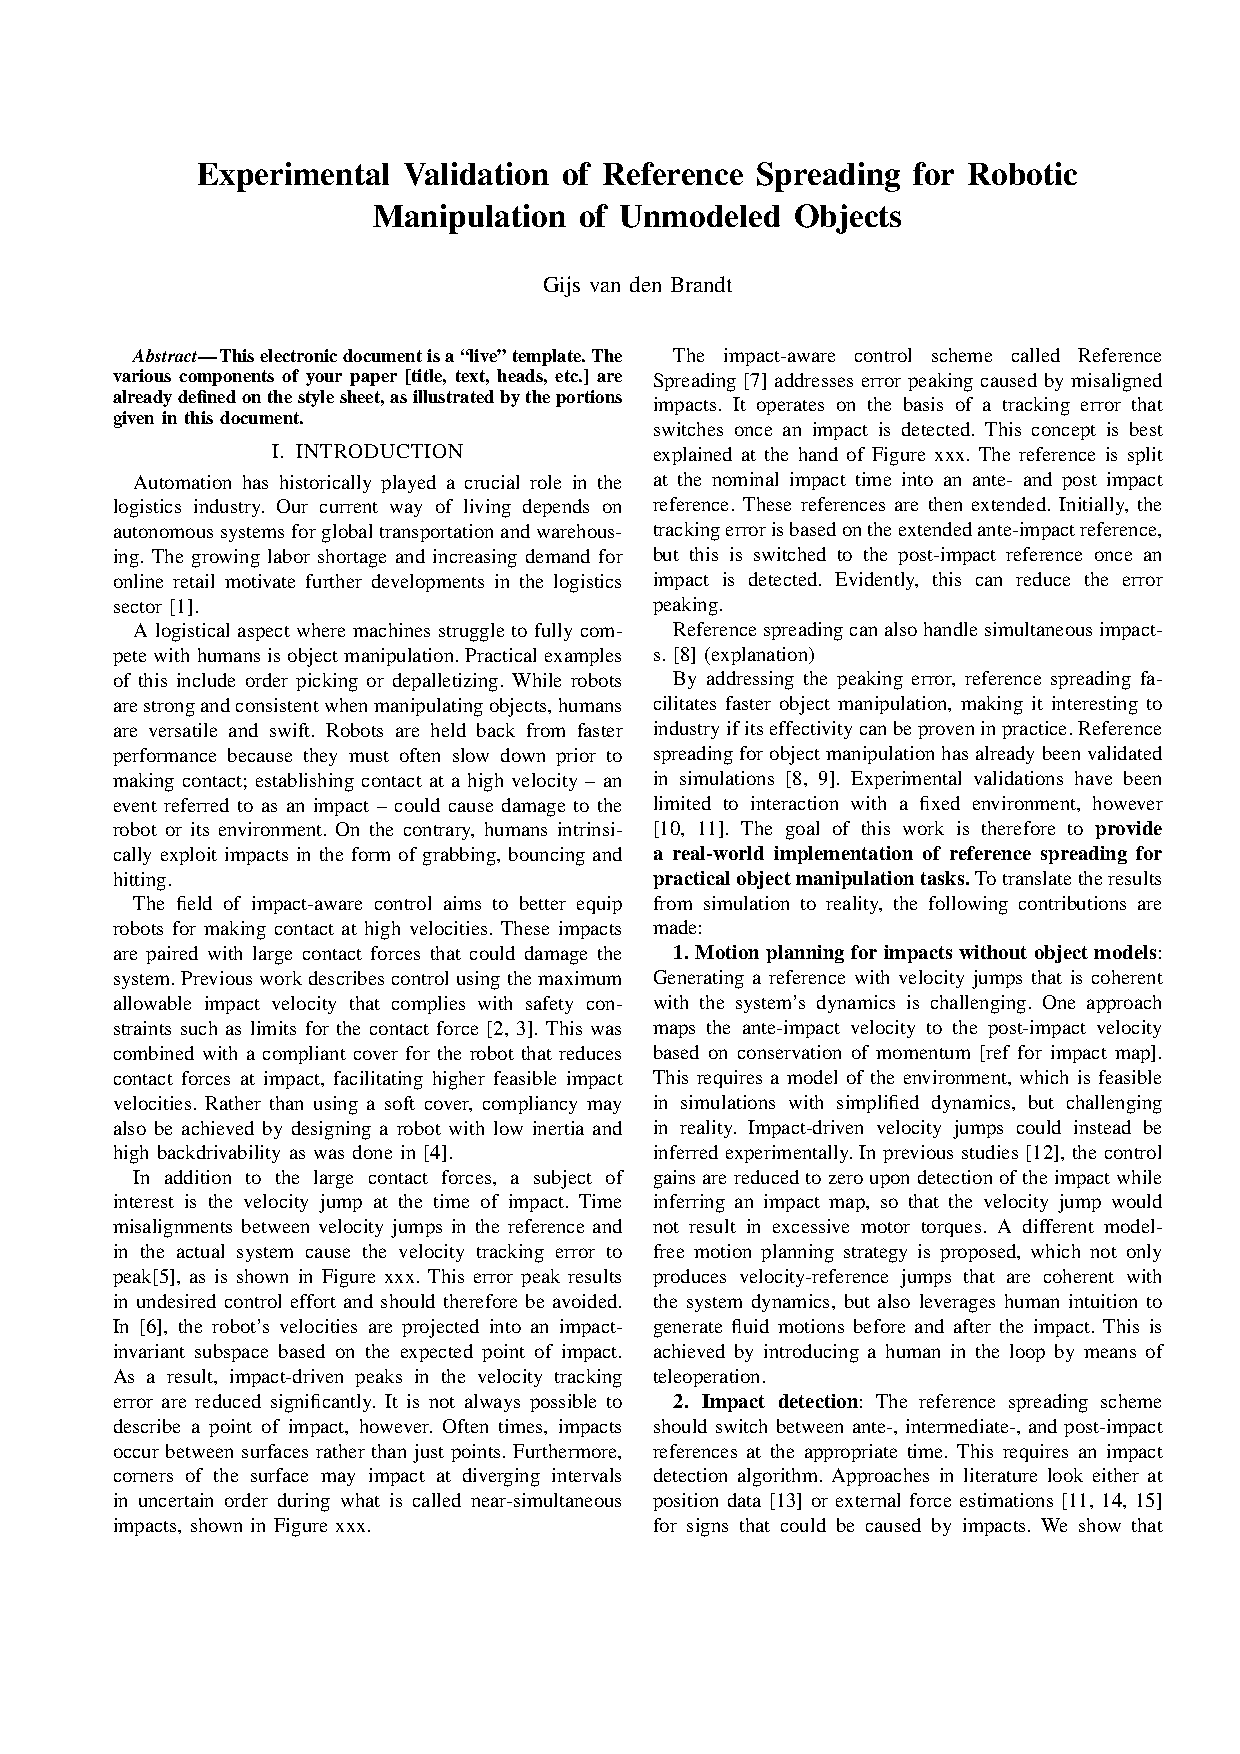
\includepdf[pages=-]{PaperPreliminary.pdf}
% BIBLIOGRAPHY

  % \newpage
  % \addcontentsline{toc}{chapter}{References}
  % \printbibliography[title=References]

  % \newpage
  % \thispagestyle{empty} \ \newpage


\end{document}